\chapter{State of the Art}
\label{sec:stateoftheart}
In this chapter we present several path planning methods that can be
applied to the problem described above. First we will introduce variations of
the Rapidly-Exploring Random Tree (RRT), a probabilistic method that builds a
tree along the free configuration space until it reaches the goal state. This
family of planners is fast at finding solutions, but the solutions are far from
optimal, and must be post-processed for shortening, smoothing or other qualities
that might be desirable in each particular problem. Furthermore, replanning RRTs
are costly in terms of computation time. We then introduce an
evolutionary planner with somewhat opposite qualities: It is slow in finding
feasible solutions in difficult maps, but efficient at replanning when a
feasible solution has already been found. It can also optimize the solution
according to any given fitness function without the need for a post-processing
step.
\section{Rapidly-Exploring Random Tree}
\label{sec:RRT}
One of the most successful probabilistic methods for offline path planning
currently in use is the Rapidly-Exploring Random Tree (RRT), a single-query planner for
static environments, first introduced in~%
\cite{Lavalle98}. RRTs works towards finding a continuous path from a state
\(q_{\text{init}}\) to a state \(q_{\text{goal}}\) in the free configuration
space \(C_{\text{free}}\) by
building a tree rooted at \(q_{\text{init}}\). A new state \(q_{\text{rand}}\) is uniformly
sampled at random from the configuration space \(C\). Then the nearest node,
\(q_{\text{near}}\), in
the tree is located, and if \(q_{\text{rand}}\) and the shortest path from
\(q_{\text{rand}}\) to
\(q_{\text{near}}\) are in \(C_{\text{free}}\), then \(q_{\text{rand}}\) is added to the tree (algorithm~%
\ref{alg:buildrrt}). The tree
growth is stopped when a node is found near \(q_{\text{goal}}\). To speed up convergence,
the search is usually biased to \(q_{\text{goal}}\) with a small probability.

In~\cite{Kuffner00}, two new features are added to RRT. First, the EXTEND
function (algorithm~\ref{alg:extend}) is introduced, which instead of trying
to add \(q_{\text{rand}}\) directly to
the tree, makes a motion towards \(q_{\text{rand}}\) and tests for collisions.

\begin{algorithm}[ht!]
    \caption{$\operatorname{BuildRRT}(q_{\text{init}},q_{\text{goal}})$}
    \label{alg:buildrrt}
    \begin{algorithmic}[1]
        \STATE{\(T \leftarrow \text{empty tree}\)}
        \STATE \(T.\operatorname{init}(q_{\text{init}})\)
        \WHILE {\(\operatorname{Distance}(T,q_{\text{goal}})> \text{threshold}\)}
            \STATE \(q_{\text{rand}} \leftarrow \operatorname{RandomConfig}()\)
            \STATE \(\operatorname{Extend}(T,q_{\text{rand}})\)
        \ENDWHILE
        \RETURN \(T\)
    \end{algorithmic}
\end{algorithm}

\begin{algorithm}[ht!]
    \caption{$\operatorname{Extend}(T,q)$}
    \label{alg:extend}
    \begin{algorithmic}[1]
        \STATE \(q_{\text{near}} \leftarrow \operatorname{NearestNeighbor}(q,T)\)
        \IF{\(\operatorname{NewConfig}(q,q_{\text{near}},q_{\text{new}})\)}
            \STATE \(T.\operatorname{add\_vertex}(q_{\text{new}})\)
            \STATE \(T.\operatorname{add\_edge}(q_{\text{near}},q_{\text{new}})\)
            \IF{\(q_{\text{new}} = q\)}
                \RETURN Reached
            \ELSE
                \RETURN Advanced
            \ENDIF
        \ENDIF
        \RETURN Trapped
    \end{algorithmic}
\end{algorithm}
Then a
greedier approach is introduced (the CONNECT function, shown in algorithms~%
\ref{alg:rrtconnectplanner} and~%
\ref{alg:connect}), which repeats EXTEND until
an obstacle is reached. This ensures that most of the time we
will be adding states to the tree, instead of just rejecting new random states.
The second extension is the use of two trees, rooted at \(q_{\text{init}}\) and
\(q_{\text{goal}}\), which are grown towards each other (see figure~%
\ref{fig:rrt}). This significantly decreases the
time needed to find a path.

\begin{figure}[ht!]
\begin{center}
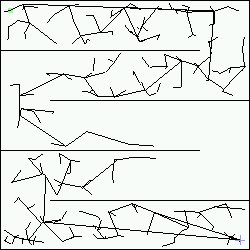
\includegraphics[width=0.4\textwidth]{images/RRT}
\caption{RRT during execution}
\label{fig:rrt}
\end{center}
\end{figure}

\begin{algorithm}[ht!]
    \caption{$\operatorname{RRTConnectPlanner}(q_{\text{init}},q_{\text{goal}})$}
    \label{alg:rrtconnectplanner}
    \begin{algorithmic}[1]
        \STATE \(T_a \leftarrow \text{tree rooted at \(q_{\text{init}}\)}\)
        \STATE \(T_b \leftarrow \text{tree rooted at \(q_{\text{goal}}\)}\)
        \STATE \(T_a.\operatorname{init}(q_{\text{init}})\)
        \STATE \(T_b.\operatorname{init}(q_{\text{goal}})\)
        \FOR{\(k=1\) to \(K\)}
            \STATE \(q_{\text{rand}} \leftarrow \operatorname{RandomConfig}()\)
            \IF{\textbf{not} (\(\operatorname{Extend}(T_a,q_{\text{rand}})=\text{Trapped}\))}
                \IF{\(\operatorname{Connect}(T_b,q_{\text{new}})=\text{Reached}\)}
                    \RETURN \(\operatorname{Path}(T_a,T_b)\)
                \ENDIF
            \ENDIF
            \STATE \(\operatorname{Swap}(T_a,T_b)\)
        \ENDFOR
        \RETURN Failure
    \end{algorithmic}
\end{algorithm}

\begin{algorithm}[ht!]
    \caption{$\operatorname{Connect}(T,q)$}
    \label{alg:connect}
    \begin{algorithmic}[1]
        \REPEAT
            \STATE \(S \leftarrow \operatorname{Extend}(T,q)\)
        \UNTIL{\((S \ne \text{Advanced})\)}
    \end{algorithmic}
\end{algorithm}

\section{Retraction-Based RRT Planner}
\label{sec:RRRT}
The Retraction-based RRT Planner presented in~\cite{Zhang08} aims at
improving the performance of the standard offline RRT in static
environments with narrow passages. The basic idea of the
\(\operatorname{Optimize}(q_r,q_n)\)
function in algorithm~%
\ref{alg:rrrt} is to iteratively retract a randomly generated
configuration
that is in \(C_{\text{obs}}\) to the closest boundary point in
\(C_{\text{free}}\). So, instead of
using the standard extension that tries to extend in a straight line from
\(q_{\text{near}}\) to \(q_{\text{rand}}\), it extends from \(q_{\text{near}}\) to the closest point in
% Fixme: extension ... extends ... extend
\(C_{\text{free}}\) to \(q_{\text{rand}}\). This gives more samples in narrow passages. This
technique could easily be applied to on-line RRT planners.
\begin{algorithm}[ht!]
\caption{Retraction-based RRT Extension}
\label{alg:rrrt}
\begin{algorithmic}[1]
    \STATE \(q_r \leftarrow \text{a random configuration in \(C_{\text{space}}\)}\)
    \STATE \(q_n \leftarrow \text{the nearest neighbor of \(q_r\) in \(T\)}\)
    \IF{\(\operatorname{CollisionFree}(q_n,q_r)\)}
        \STATE \(T.\operatorname{addVertex}(q_r)\)
        \STATE \(T.\operatorname{addEdge}(q_n,q_r)\)
    \ELSE
        \STATE \(S \leftarrow \operatorname{Optimize}(q_r,q_n)\)
        \FORALL{\(q_i \in S\)}
            \STATE Standard RRT Extension\((T,q_i)\)
        \ENDFOR
    \ENDIF
    \RETURN $T$
\end{algorithmic}
\end{algorithm}

\section{Execution Extended RRT}
\label{sec:ERRT}
The Execution Extended RRT presented in~\cite{Bruce02} introduces two
extensions to RRT to build an on-line planner, the waypoint cache and adaptive
cost penalty search, which
improve re-planning efficiency and the quality of generated paths. ERRT uses
a \mbox{kd-tree}~(see section~\ref{sec:kd-tree}) to speed nearest neighbor look-up, and does not use
bidirectional search. The waypoint cache is implemented by keeping a constant
size array of states, and whenever a plan is found, all the states in the plan
are placed in the cache with random replacement. Then, when the tree is no
longer valid, a new tree must be grown, and there are three
possibilities for choosing a new target state, as shown in algorithm
\ref{alg:choosetarget}, which is used instead of
\(\operatorname{RandomConfig}()\) in previous
algorithms. With probability
P[\textit{goal}], the goal is chosen as the target; with probability
P[\textit{waypoint}], a random waypoint is chosen, and with the remaining
probability a uniform state is chosen as before. In~\cite{Bruce02} the values used
are P[\textit{goal}]$=0.1$ and P[\textit{waypoint}]$=0.6$.

Another extension is adaptive cost penalty search, where the planner adaptively
modified a parameter to help it find shorter paths. A value of 1 for beta will
always extend from the root node, while a value of 0 is equivalent to the
original algorithm. However, the paper~\cite{Bruce02} lacks
implementation details and experimental results on this extension.

\begin{algorithm}[ht!]
    \caption{$\operatorname{ChooseTarget}(q,{\text{goal}})$}
    \label{alg:choosetarget}
    \begin{algorithmic}[1]
        \STATE \(p \leftarrow \operatorname{UniformRandom}(0.0,1.0)\)
        \STATE \(i \leftarrow \operatorname{UniformRandom}(0.0,\text{NumWayPoints})\)
        \IF{\(0 < p < \text{GoalProb}\)}
            \RETURN \(q_{\text{goal}}\)
        \ELSIF{\(\text{GoalProb}<p<\text{GoalProb}+\text{WayPointProb}\)}
            \RETURN \(\text{WayPointCache}[i]\)
        \ELSIF{\(\text{GoalProb}+\text{WayPointProb}<p<1\)}
            \RETURN \(\text{RandomConfig}()\)
        \ENDIF
    \end{algorithmic}
\end{algorithm}

\section{Dynamic RRT}
\label{sec:DRRT}
The Dynamic Rapidly-Exploring Random Tree described in~\cite{Ferguson06} is a
probabilistic analog to the widely used D* family of algorithms. It works by
growing a tree from \(q_{\text{goal}}\) to \(q_{\text{init}}\), as shown in algorithm
\ref{alg:drrt}. This has the advantage that the
root of the tree does not have to be moved during the lifetime of the planning
and execution. In some problem classes the robot has limited range
sensors, thus moving or newly appearing obstacles will be near the robot, not
near the goal. In general this strategy attempts to trim smaller branches that are
farther away from the root. When new information concerning the configuration space is
received, the algorithm removes the newly-invalid branches of the
tree (algorithms~\ref{alg:trimrrt} and~\ref{alg:invalidatenodes}), and
grows the remaining tree, focusing, with a certain probability (empirically tuned
to $0.4$ in~\cite{Ferguson06}) to a vicinity of the recently trimmed branches,
by using the waypoint
cache of the ERRT~(algorithm~\ref{alg:choosetarget}). In experiments presented
in~\cite{Ferguson06} DRRT vastly outperforms ERRT.

\begin{algorithm}[ht!]
    \caption{$\operatorname{DRRT}()$}
    \label{alg:drrt}
    \begin{algorithmic}[1]
        \STATE \(q_{\text{robot}} \leftarrow \text{the current robot position}\)
        \STATE \(T \leftarrow \operatorname{BuildRRT}(q_{\text{goal}},q_{\text{robot}})\)
        \WHILE{\(q_{\text{robot}} \neq q_{\text{goal}}\)}
            \STATE \(q_{\text{next}}  \leftarrow \operatorname{Parent}(q_{\text{robot}})\)
            \STATE Move from \(q_{\text{robot}}\) to \(q_{\text{next}}\)
            \FORALL{obstacles that changed $O$}
                \STATE \(\operatorname{InvalidateNodes}(O)\)
            \ENDFOR
            \IF{Solution path contains an invalid node}
                \STATE \(\operatorname{ReGrowRRT}()\)
            \ENDIF
        \ENDWHILE
    \end{algorithmic}
\end{algorithm}

\begin{algorithm}[ht!]
\caption{$\operatorname{ReGrowRRT}()$}
\label{alg:regrowrrt}
\begin{algorithmic}[1]
    \STATE \(\operatorname{TrimRRT}()\)
    \STATE \(\operatorname{GrowRRT}()\)
\end{algorithmic}
\end{algorithm}

\begin{algorithm}[ht!]
\caption{$\operatorname{TrimRRT}()$}
\label{alg:trimrrt}
\begin{algorithmic}[1]
    \STATE \(S \leftarrow \emptyset, i \leftarrow 1\)
    \WHILE{\(i < T.\operatorname{size}()\)}
        \STATE \(q_i \leftarrow  T.\operatorname{node}(i)\)
        \STATE \(q_p \leftarrow  \operatorname{Parent}(q_i)\)
        \IF{\(q_p.\text{flag} = \text{INVALID}\)}
            \STATE \(q_i.\text{flag} \leftarrow  \text{INVALID}\)
        \ENDIF
        \IF{\(q_i.\text{flag} \neq \text{INVALID}\)}
            \STATE \(S \leftarrow  S \bigcup \{q_i\}\)
        \ENDIF
        \STATE \(i \leftarrow i+1\)
    \ENDWHILE
    \STATE \(T \leftarrow  \operatorname{CreateTreeFromNodes}(S)\)
\end{algorithmic}
\end{algorithm}


\begin{algorithm}[ht!]
\caption{$\operatorname{InvalidateNodes}(obstacle)$}
\label{alg:invalidatenodes}
\begin{algorithmic}[1]
    \STATE \(E \leftarrow \operatorname{FindAffectedEdges}(\text{obstacle})\)
    \FORALL{\(e \in E\)}
        \STATE \(q_e \leftarrow  \operatorname{ChildEndpointNode}(e)\)
        \STATE \(q_e.\text{flag} \leftarrow  \text{INVALID}\)
    \ENDFOR
\end{algorithmic}
\end{algorithm}

\section{Multipartite RRT}
\label{sec:MPRRT}
Multipartite RRT presented in~\cite{Zucker07} is another RRT variant which
supports planning in unknown or dynamic environments. MP-RRT maintains a
forest $F$ of disconnected sub-trees which lie in \(C_{\text{free}}\), but which are not
connected to the root node \(q_{\text{root}}\) of $T$, the main tree. At the start of a
given planning iteration, any nodes of $T$ and $F$ which are no longer valid are
deleted, and any disconnected sub-trees which are created as a result are placed
into $F$~(as seen in algorithms~\ref{alg:mprrtsearch} and~\ref{alg:pruneandprepend}).
With given probabilities,
the algorithm tries to connect $T$ to a
new random state, to the goal state, or to the root of a tree in $F$ (algorithm~%
\ref{alg:selectsample}). In~%
\cite{Zucker07}, a simple greedy smoothing heuristic is used, that tries to
shorten paths by skipping intermediate nodes. The MP-RRT
is compared to an iterated RRT, ERRT and DRRT, in 2D, 3D and 4D problems, with
and without smoothing. For most of the experiments, MP-RRT modestly outperforms
the other algorithms, but in the 4D case with smoothing, the performance gap in
favor of MP-RRT is much larger. The authors explained this fact due to MP-RRT
being able to construct much more robust plans in the face of dynamic obstacle
motion. Another algorithm that utilizes the concept of forests is
Reconfigurable Random Forests (RRF) presented in~\cite{Li02}, but without the
success of MP-RRT.

\begin{algorithm}[ht!]
\caption{$\operatorname{MPRRTSearch}(q_{\text{init}})$}
\label{alg:mprrtsearch}
\begin{algorithmic}[1]
    \STATE \(T \leftarrow \text{the previous search tree, if any}\)
    \STATE \(F \leftarrow \text{the previous forest of disconnected sub-trees}\)
    \STATE \(q_{\text{init}} \leftarrow \text{the initial state}\)
    \IF{\(T=\emptyset\)}
        \STATE \(q_{\text{root}} \leftarrow  q_{\text{init}}\)
        \STATE \(\operatorname{Insert}(q_{\text{root}},T)\)
    \ELSE
        \STATE \(\operatorname{PruneAndPrepend}(T,F,q_{\text{init}})\)
        \IF{\(\operatorname{TreeHasGoal}(T)\)}
            \RETURN \TRUE
        \ENDIF
    \ENDIF
    \WHILE{search time/space remaining}
        \STATE \(q_{\text{new}} \leftarrow  \operatorname{SelectSample}(F)\)
        \STATE \(q_{\text{near}} \leftarrow  \operatorname{NearestNeighbor}(q_{\text{new},T})\)
        \IF{\(q_{\text{new}}\in F\)}
            \STATE \(b_{\text{connect}} \leftarrow  \operatorname{Connect}(q_{\text{near}},q_{\text{new}})\)
            \IF{\(b_{\text{connect}}\) \textbf{and}  \(\operatorname{TreeHasGoal}(T)\)}
                \RETURN \TRUE
            \ENDIF
        \ELSE
            \STATE \(b_{\text{extend}} \leftarrow   \operatorname{Extend}(q_{\text{near}},q_{\text{new}})\)
            \IF{\(b_{\text{extend}}\) \textbf{and} \(\operatorname{IsGoal}(q_{\text{new}})\)}
                \RETURN \TRUE
            \ENDIF
        \ENDIF
    \ENDWHILE
    \RETURN \FALSE
\end{algorithmic}
\end{algorithm}

\begin{algorithm}[ht!]
\caption{$\operatorname{PruneAndPrepend}(T,F,q_{\text{init}})$}
\label{alg:pruneandprepend}
\begin{algorithmic}[1]
    \FORALL{\(q\in T,F\)}
        \IF{\textbf{not} \(\operatorname{NodeValid}(q)\)}
            \STATE \(\operatorname{KillNode}(q)\)
        \ELSIF{\textbf{not} \(\operatorname{ActionValid}(q)\)}
            \STATE \(\operatorname{SplitEdge}(q)\)
        \ENDIF
    \ENDFOR
    \IF{\textbf{not} \(T=\emptyset\) \textbf{and} \(q_{\text{root}} \neq q_{\text{init}}\)}
        \IF{\textbf{not} \(\operatorname{ReRoot}(T,q_{\text{init}})\)}
            \STATE \(F \leftarrow  F \bigcup T\)
            \STATE \(T.\operatorname{init}(q_{\text{init}})\)
        \ENDIF
    \ENDIF
\end{algorithmic}
\end{algorithm}

\begin{algorithm}[ht!]
\caption{$\operatorname{SelectSample}(F)$}
\label{alg:selectsample}
\begin{algorithmic}[1]
    \STATE \(p \leftarrow  \operatorname{Random}(0,1)\)
    \IF{\(p<p_{\text{goal}}\)}
        \STATE \(q_{\text{new}} \leftarrow q_{\text{goal}}\)
    \ELSIF{\(p<(p_{\text{goal}}+p_{\text{forest}})\) \textbf{and not} \(\operatorname{Empty}(F)\)}
        \STATE \(q_{\text{new}} \leftarrow  q \in \operatorname{SubTreeRoots}(F)\)
    \ELSE
        \STATE \(q_{\text{new}} \leftarrow  \operatorname{RandomState}()\)
    \ENDIF
    \RETURN \(q_{\text{new}}\)
\end{algorithmic}
\end{algorithm}

\section{Rapidly Exploring Evolutionary Tree}
\label{sec:RET}
The Rapidly Exploring Evolutionary Tree, introduced in~\cite{Martin07} uses a
bidirectional RRT and a \mbox{kd-tree}~(see section~\ref{sec:kd-tree}) for efficient
nearest neighbor search. The
modifications to the \(\operatorname{Extend}()\) function are shown in algorithm
\ref{alg:extendtotarget}. The
re-balancing of a \mbox{kd-tree} is costly, and in this paper a simple threshold on the
number of nodes added before re-balancing was used. The authors suggest using the
method described in~\cite{Atramentov02} and used in~\cite{Bruce02} to improve
the search speed. The novelty in this algorithm comes from the introduction of
an evolutionary algorithm~\cite{Back97} that builds a population of biases for the RRTs. The
genotype of the evolutionary algorithm consists of a single robot configuration for each tree. This
configuration is sampled instead of the uniform distribution. To balance
exploration and exploitation, the evolutionary algorithm was designed with 50\% elitism. The fitness
function is related to the number of left and right branches traversed during
the insertion of a new node in the \mbox{kd-tree}. The goal is to introduce a bias to
the RRT algorithm which shows preference to nodes created away from the center
of the tree. The authors suggest combining RET with DRRT or MP-RRT.

\begin{algorithm}[ht!]
\caption{$\operatorname{ExtendToTarget}(T)$}
\label{alg:extendtotarget}
\begin{algorithmic}[1]
    \STATE \textbf{static} $p$: population, \(inc \leftarrow 1\)
    \STATE \(p'\): temporary population
    \IF{\(\text{inc}>\operatorname{length}(p)\)}
        \STATE \(\operatorname{SortByFitness}(p)\)
        \STATE \(p' \leftarrow  \text{null}\)
        \FORALL{\(i \in p\)}
            \IF{i is in upper 50\%}
                \STATE \(\operatorname{AddIndividual}(i,p')\)
            \ELSE
                \STATE \(i \leftarrow  \operatorname{RandomState}()\)
                \STATE \(\operatorname{AddIndividual}(i,p')\)
            \ENDIF
        \ENDFOR
        \STATE \(p \leftarrow  p'\)
        \STATE \(\text{inc} \leftarrow  1\)
    \ENDIF
    \STATE \(q_r \leftarrow  p(\text{inc})\)
    \STATE \(q_{\text{near}} \leftarrow   \operatorname{Nearest}(T,q_r)\)
    \STATE \(q_{\text{new}} \leftarrow  \operatorname{Extend}(T,q_{\text{near}})\)
    \IF{\(q_{\text{new}} \neq \emptyset\)}
        \STATE \(\operatorname{AddNode}(T,q_{\text{new}})\)
        \STATE \(\operatorname{AssignFitness}(p(\text{inc}),\operatorname{fitness}(q_{\text{new}})\)
    \ELSE
        \STATE \(\operatorname{AssignFitness}(p(\text{inc}),0)\)
    \ENDIF
    \RETURN \(q_{\text{new}}\)
\end{algorithmic}
\end{algorithm}

\section{Multidimensional Binary Search Trees}
\label{sec:kd-tree}
The kd-tree, first introduced in~\cite{Bentley75}, is a binary tree in which every 
node is a \mbox{k-dimensional} point. Every
non-leaf node generates a splitting hyperplane that divides the space into two
subspaces. In the RRT algorithm, the number of points grows incrementally,
unbalancing the tree, thus slowing nearest-neighbor queries. Re-balancing a kd-tree
is costly, so in~\cite{Atramentov02} the authors present another approach:
A vector of trees is constructed, where for $n$ points there is a tree that
contains $2^i$ points for each $"1"$ in the $i^{th}$ place of the binary
representation of $n$. As bits are cleared in the representation due to
increasing $n$, the trees are deleted, and the points are included in a tree
that corresponds to the higher-order bit which is changed to $"1"$. This general
scheme incurs in logarithmic-time overhead, regardless of dimension. Experiments
show a substantial performance increase compared to a naive brute-force approach.

\section{Evolutionary Planner/Navigator}
\label{sec:EP/N}
An evolutionary algorithm~\cite{Back97} is a generic population-based meta-heuristic
optimization algorithm. It is inspired in biological evolution, using methods
such as individual selection, reproduction and mutation. The population is
composed of candidate solutions and they are evaluated according to a fitness
function.

The Evolutionary Planner/Navigator presented in~\cite{Xiao96},~\cite{Xiao97}, and~
\cite{Trojanowski97} is an evolutionary
algorithm for path finding in dynamic environments. A high level description is
shown in algorithm~\ref{alg:epn}. A difference with RRT is
that it can optimize the path according to any fitness function
defined (length, smoothness, etc), without the need for a post-processing step.
Experimental tests have shown it has
good performance for sparse maps, but no so much for difficult maps with narrow
passages or too crowded with obstacles. However, when a feasible path is found,
it is very efficient at optimizing it and adapting to the dynamic obstacles.
\begin{algorithm}[ht!]
\caption{EP/N}
\label{alg:epn}
\begin{algorithmic}[1]
    \STATE \(P(t)\): population at generation \(t\)
    \STATE \(t \leftarrow 0\)
    \STATE \(\operatorname{Initialize}(P(t))\)
    \STATE \(\operatorname{Evaluate}(P(t))\)
    \WHILE{(\textbf{not} termination-condition)}
        \STATE \(t \leftarrow t + 1\)
        \STATE Select operator $o_j$ with probability $p_j$
        \STATE Select parent(s) from $P(t)$
        \STATE Produce offspring applying $o_j$ to selected parent(s)
        \STATE Evaluate offspring
        \STATE Replace worst individual in $P(t)$ by new offspring
        \STATE Select best individual $p$ from $P(t)$
        \IF{\(\operatorname{Feasible}(p)\)}
            \STATE Move along path \(p\)
            \STATE Update all individuals in \(P(t)\) with current position
            \IF{changes in environment}
                \STATE Update map
            \ENDIF
            \STATE \(\operatorname{Evaluate}(P(t))\)
        \ENDIF
        \STATE \(t \leftarrow t + 1\)
    \ENDWHILE
\end{algorithmic}
\end{algorithm}
Every individual in the population is a sequence of nodes, representing
nodes in a path consisting of straight-line segments. Each node consists of an
$(x,y)$ pair and a state variable $b$ with information about the feasibility of
the point and the path segment connecting it to the next point. Individuals have
variable length.

Since a path $p$ can be either feasible or unfeasible, two evaluation functions
are used. For feasible paths (equation~\ref{eq:fitness}), the goal is to minimize distance traveled,
maintain a smooth trajectory and satisfy a clearance requirement (the robot
should not approach the obstacles too closely). For unfeasible paths, we use
equation~\ref{eq:unfeasible}, taken from~\cite{Xiao97-2}, where $\mu$ is the number 
of intersections of a whole path with obstacles and $\eta$ is the average number
of intersections per unfeasible segment.

\begin{equation}
\label{eq:fitness}
\operatorname{eval}_f(p)=w_d\cdot \operatorname{dist}(p) + w_s\cdot \operatorname{smooth}(p)+w_c\cdot \operatorname{clear}(p)
\end{equation}

\begin{equation}
\label{eq:unfeasible}
\operatorname{eval}_u(p)= \mu + \eta
\end{equation}

\begin{figure}[ht!]
\begin{center}
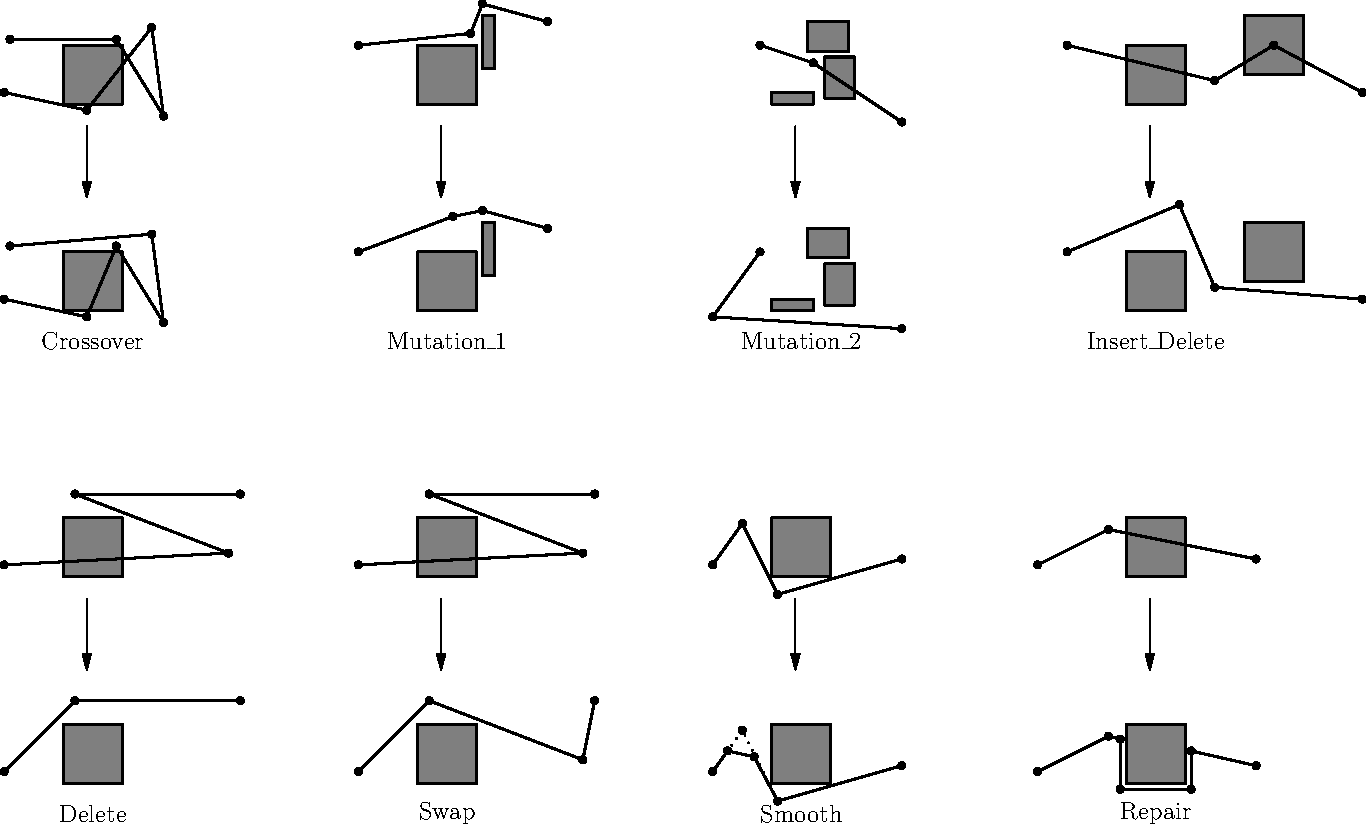
\includegraphics[width=0.9\textwidth]{images/operators.pdf}
\caption{The roles of the genetic operators}
\label{fig:operators}
\end{center}
\end{figure}
EP/N uses eight different operators, as shown in figure~%
\ref{fig:operators} (description taken from~\cite{Xiao96}):
\begin{description}
\item{\it Crossover:} Recombines two (parent) paths into two new paths. The
parent paths are divided randomly into two parts respectively and recombined:
The first part of the first path with the second part of the second path, and
the first part of the second path with the second part of the first path. Note
that there can be different numbers of nodes in the two parent paths.
\item{\it Mutate\_1:} Used to fine tune node coordinates in a
feasible path for shape adjustment. This operator randomly adjusts node
coordinates within some local clearance of the path so that the path remains
feasible afterwards.
\item{\it Mutate\_2:} Used for large random changes of node coordinates in
a path, which can be either feasible or unfeasible.
\item{\it Insert-Delete:} Operates on an unfeasible path by inserting
randomly generated new nodes into unfeasible path segments and deleting
unfeasible nodes (i.e., path nodes that are inside obstacles).
\item{\it Delete:} Deletes nodes from a path, which can be
either feasible or unfeasible. If the path is unfeasible,
the deletion is done randomly. Otherwise, the operator
decides whether a node should definitely be deleted
based on some heuristic knowledge, and if a node is
not definitely deletable, its deletion will be random.
\item{\it Swap:} Swaps the coordinates of randomly selected
adjacent nodes in a path, which can be either feasible
or unfeasible.
\item{\it Smooth:} Smoothens turns of a feasible path by ``cutting corners,''
i.e., for a selected node, the operator
inserts two new nodes on the two path segments connected to that node
respectively and deletes that selected node. The nodes with sharper turns are
more likely to be selected.
\item{\it Repair:} Repairs a randomly selected unfeasible segment
in a path by ``pulling'' the segment around its
intersecting obstacle.
\end{description}
The probabilities of using each operator is set randomly at the beginning, and
then are updated according to the success ratio of each operator, so more
successful operators are used more often, and automatically chosen according to
the instance of the problem, eliminating the difficult problem of hand tuning
the probabilities.

In~\cite{Trojanowski97}, the authors include a memory buffer for each
individual to store good paths from its ancestors, which gave a small performance
gain.

In~\cite{Elshamli04}, the authors propose strategies for improving the
stability
and controlling population diversity for a simplified version of the EP/N.
An improvement proposed by the authors in~\cite{Xiao97} is using heuristics for the initial
population, instead of random initialization. We will consider this improvement
in section~\ref{sec:RRT-EP/N}.

Other evolutionary algorithms have also been proposed for similar problems, in~%
\cite{Nagib04} a binary genetic algorithm is used for an offline planner, and~%
\cite{Nikolos03} presents an algorithm to generate curved trajectories in 3D
space for an unmanned aerial vehicle.

EP/N has been adapted to an 8-connected grid model in~%
\cite{Alfaro08} (with previous work in~\cite{Alfaro05} and~\cite{Alfaro05-2}).
The authors study two different crossover operators and four asexual operators.
Experimental results for this new algorithm (EvP) in static unknown environments
show that it is faster than EP/N.
